\section{Introduction}
In reinforcement learning (RL), an agent perceives and reacts to consecutive states of its environment to maximize long-term cumulative expected reward \cite{book:sutton1998introduction}. %in a receding-horizon framework.
One key challenge to the widespread deployment of RL in safety-critical systems is ensuring that an RL agent's policies are safe, especially when the system environment or dynamics are a black box and subject to noise \cite{mihatsch2002risk,garcia2015comprehensive}. %garcia2020teaching, koppejan2011neuroevolutionary,
In this work, we consider RL for guaranteed-safe navigation of mobile robots, such as autonomous cars or delivery drones, where safety means collision avoidance.
We leverage RL to plan complex action sequences in concert with data-driven reachability analysis to guarantee safety for a black-box system.

\begin{figure}[t]
    \centering
    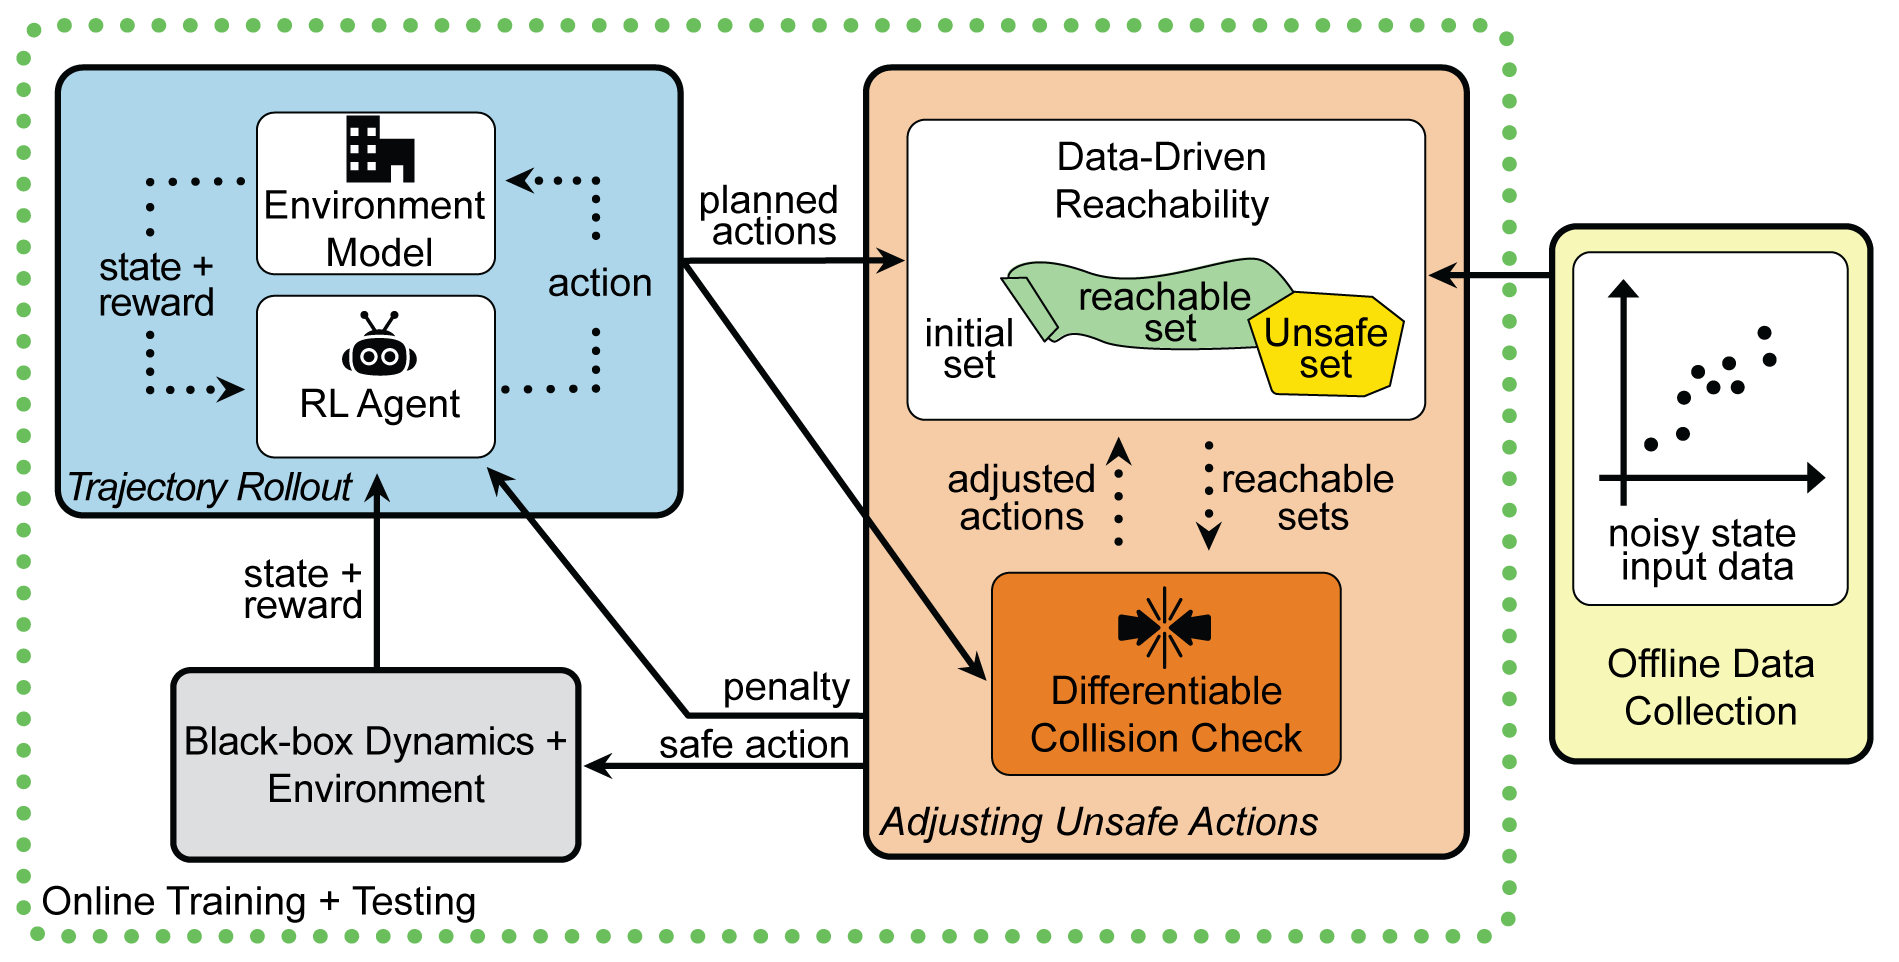
\includegraphics[width=\columnwidth]{Figures/20210922_BRSL-04.png}
    \vspace{-5mm}
    \caption{Overview of the proposed BRSL method (\href{https://youtube.com/playlist?list=PL7bkcpwNaUjz-S1b5KBzpgCZ1SP4DXsoi}{\textcolor{blue}{link to video}}).
    Given data collected offline (in yellow, right), we perform online safe training and deployment of an RL agent.
    The RL agent creates trajectory plans for a robot in a receding-horizon way as follows.
    Each planning iteration is one clockwise loop in the green dashed box.
    First (blue, top left), the agent predicts a possible future trajectory by rolling out its current policy with an ensemble of neural networks trained online to model the black-box environment (grey, bottom left).
    Second (orange, middle), the candidate plan is \emph{adjusted} to ensure safety using data-driven reachability and a constrained, differentiable method of collision-checking our robot's reachable sets.
    We execute a failsafe maneuver if the collision check is infeasible.
    Finally, the new safe plan is passed to the robot, and a penalty is passed to the RL agent for choosing unsafe action.}
    \label{fig:framework}
    \vspace{-6mm}
\end{figure}










\subsection{Related Work} \label{sec:related}
%\textbf{Related Work.}
%Safety has long been of interest in RL research. %Unlike traditional RL, 
Safe RL aims to learn policies that maximize expected reward on a task while respecting safety constraints during both learning and deployment \cite{garcia2015comprehensive}. 
Existing methods can be roughly classified as \emph{objective-based} or \emph{exploration-based}, depending on how safety is formulated.
We first discuss these categories, then the specific case of mobile robot navigation, which we use to evaluate our proposed method.

Objective-based methods encourage safety by penalizing constraint violations in the objective.
This can be done by relating cumulative reward to the system's risk, such as the probability of visiting error states \cite{geibel2005risk}.
In practice, this results in an RL agent attempting to minimize an empirical risk measure (that is, an approximation of the probability of entering a dangerous or undesired state).
Similarly, one can penalize the probability of losing reward (by visiting an unsafe state) for a given action \cite{mihatsch2002risk}, in which case the agent minimizes temporal differences in the reward and thus also minimizes risk.
Another approach is to restrict policies to be ergodic with high probability, meaning any state can eventually be reached from any other state \cite{moldovan2012safe}.
This is a more general problem, which comes at a cost: feasible safe policies do not always exist, and the algorithms are far more complex. 
While these methods can make an agent prefer safe actions, they cannot guarantee safety during training or deployment.
Another group of objective-based algorithms aims to modify the Markov Decision Process (MDP) that the RL agent tries to optimize.
Some model safe optimization problems as maximizing an unknown expected reward function \cite{pmlr-v37-sui15}.
However, they exploit regularity assumptions on the function wherein similar decisions are associated with similar rewards.
They also assume the bandit setting, where decisions do not cause state transitions.
% Others utilize constrained MDPs to enforce safety \cite{altman1999constrained}.
% These can be broadly classified as either offline or online approaches.
% Offline approaches \cite{achiam2017constrained,bharadhwaj2021conservative} collect data first, then perform the optimization.
% These methods can be quite conservative and hard to scale.
% Online methods \cite{BORKAR2005207,chow2017riskconstrained,bohez2019value}, on the other hand, couple both the data collection and optimization.
% However, they do not guarantee safety in training.
Others utilize constrained MDPs \cite{altman1999constrained} to enforce safety in various RL settings, either online or offline.
Online methods learn by coupling the iteration of numerical optimization algorithms (such as primal-dual gradient updates) with data collection \cite{BORKAR2005207,chow2017riskconstrained,tessler2018reward,bohez2019value}.
These algorithms have also been studied in exploration-based settings \cite{ding2020provably,efroni2020explorationexploitation}.
However, they provide no guarantees on safety during training.
On the other hand, offline schemes separate optimization and data collection \cite{achiam2017constrained,bharadhwaj2021conservative}.
They conservatively enforce safety constraints on every policy iteration but are more challenging to scale up.


Exploration-based methods modify the agent's exploration process instead of its optimization criterion.
Exploration is the process of learning about unexplored states by trying random actions or actions that are not expected to yield maximum reward (for example, an $\epsilon$-greedy strategy).
However, visiting unexplored states na\"ively can harm a robot or its environment.
To avoid this, one can aim to guarantee safety during both exploration and exploitation, in both training and testing, by modifying the exploration strategy to incorporate risk metrics \cite{riskmetricsRL}.
One can also use prior knowledge as an inductive bias for the exploration process \cite{garcia2015comprehensive,neuroevolutionaryinproceedings}; for example, one can provide a finite set of demonstrations as guidance on the task \cite{abbeel2005exploration}.
\tb{
Other approaches use control theory to guide or constrain the RL agent's actions.
Most of these approaches use system models with Lyapunov or control barrier functions (CBFs) to guarantee safety (or stability) of the system \cite{molnar2021model, liu2022robot, chow2018lyapunov}.
One can also combine data-driven approaches with model-free barrier or intervention functions \cite{cheng2019end, modelfreecbfsIVM, wagener2021safe}, or use robust CBFs to model uncertain parts of a system \cite{robustCBFarticle, cbfforunmodeleddynamics}.
Although these approaches can provide strong guarantees, most assume the system is control-affine, and need prior knowledge on some or all of the system model \cite{saferlforchanginglanes,conf:modelBasedReachRL,LewEtAl2021}, which may not always be feasible.
Finally, our method is most similar to \cite{dalal2018safe}, which learns a safety signal from data offline, then uses it to adjust an RL agent's controls at runtime.
This method uses a first-order safety approximation for fast adjustment, but (as we show) can be conservative.
}
 
%\subsection{Robot Navigation using Safe RL }
\tb{
Safe navigation is a fundamental challenge in robotics, because robots typically have uncertain, nonlinear dynamics.
Classical techniques such as A$^*$ or RRT \cite[Ch. 5]{lavalle2006planning} have been proposed to solve the navigation problem without learning.
With these methods, safety has been enforced at different levels of the planning hierarchy, such as trajectory planning \cite{kousik2020bridging}, or low-level control \cite{leung2020infusing}.
More recently, however, learning-based methods have been proposed \cite{saferlforchanginglanes,conf:modelBasedReachRL,LewEtAl2021}.
Some safe RL navigation approaches depend on learning a value function of the expected time that an agent takes to reach the desired goal \cite{chen2016decentralized, chen2018socially}.
Other approaches depend on learning the actions of the robot in an end-to-end manner \cite{long2018optimally, e2efirst, tai2018socially}, meaning that the agent attempts to convert raw sensor inputs (e.g., camera or LIDAR) into actuator commands.
The key advantage of RL over traditional planners is in accelerating computation time and solution quality. %by learning from past experience.
}



\subsection{Proposed Method and Contributions}
%\textbf{Proposed Method.}
% We propose a , which guarantees safety during exploration and exploitation in RL.
\tb{We propose a Black-box Reachability-based Safety Layer (BRSL), illustrated in Fig.~\ref{fig:framework}, to enable strict safety guarantees for RL in an entirely data-driven way, addressing the above challenges of lacking robot and environment models \emph{a priori} and of enforcing safety for uncertain systems.
We note that the main advantage of BRSL is the use of data-driven methods to provide safety guarantees for black-box system dynamics.}
BRSL enforces safety by computing a system's forward reachable set, which is the union of all trajectories that the system can realize within a finite or infinite time when starting from a bounded set of initial states, subject to a set of possible input signals \cite{conf:reach1984}. 
Then, if the reachable set does not intersect with unsafe sets, the system is verified as safe, following similar arguments as in \cite{kousik2020bridging,leung2020infusing,althoffphdthesis}.

\textbf{Limitations.}
Our method requires an approximation for the upper bound of a system's Lipschitz constant, similar to \cite{LewEtAl2021,koller2018learning,alanwar2020data_conf}.
This results in a curse of dimensionality with respect to number of samples required to approximate the constant; note other sampling-based approaches scale similarly \cite{LewEtAl2021,conf:modelBasedReachRL}. 
Furthermore, we focus on a discrete-time setting, assume our robot can brake to a stop, and assume accurate perception of the robot's surroundings.
We leave continuous-time (which can be addressed with similar reachability methods to ours \cite{conf:modelBasedReachRL,althoffphdthesis}) and perception uncertainty to future work. 


% Our BRSL framework, illustrated in Fig. \ref{fig:framework}, has three components: (1) a \emph{dreaming} trajectory planner, (2) a data-driven reachability analysis technique based on \cite{alanwar2020data}, and (3) a method of adjusting unsafe actions using a novel differentiable collision check based on \cite{chung2021constrained}.
% BRSL operates as follows.
% First, offline, we collect noisy state-input data from the trajectories of the system. 
% At runtime, the RL agent generates actions in a receding-horizon way.
% In each receding-horizon iteration, BRSL performs trajectory planning using an ensemble of neural networks, trained online to mimic the environment.
% This allows the RL agent to \emph{dream} a future plan before executing it.
% Since the dreamed plan may be unsafe, we propose a novel safety layer to \emph{adjust} any unsafe actions in the plan.
% This adjustment is achieved by first computing the reachable set of the plan as a sequence of polytopes using the technique in \cite{alanwar2020data_conf}; then, by extending the differentiable polytope collision checking method in \cite{chung2021constrained}, we use constrained gradient descent to push the reachable sets out of collision and identify safe actions.

% In summary, BRSL makes the following contributions:
\textbf{Contributions.}
We show the following with BRSL:
\begin{enumerate}[leftmargin=15pt,noitemsep,partopsep=0pt,topsep=0pt,parsep=0pt]
\itemsep0em
    
    \item We propose a safety layer by integrating data-driven reachability analysis with a differentiable polytope collision check and a trajectory rollout planner.
    
    \item We demonstrate BRSL on robot navigation, where it outperforms a baseline RL agent, Reachability-based Trajectory Safeguard (RTS) \cite{conf:modelBasedReachRL}, Safe Advantage-based Intervention for Learning policies with Reinforcement (SAILR) \cite{wagener2021safe}, and Safe Exploration in Continuous Action Spaces (SECAS) \cite{dalal2018safe}.
    Our code is \href{https://github.com/Mahmoud-Selim/Safe-Reinforcement-Learning-for-Black-Box-Systems-Using-Reachability-Analysis}{\underline{\color{blue}{online}}}.
\end{enumerate}

Next, in Section \ref{sec:pb}, we provide preliminaries and formulate our safe RL problem. 
Sections \ref{sec:solu} and \ref{sec:eval} discuss and evaluate the proposed approach.
Finally, Section \ref{sec:con} presents concluding remarks and discusses future work.

% \tb{The code to recreate our findings is publicly available.}


% \footnotetext{Our code is available \href{https://github.com/Mahmoud-Selim/Safe-Reinforcement-Learning-for-Black-Box-Systems-Using-Reachability-Analysis}{online (click for link)} %\href{https://github.com/Mahmoud-Selim/Safe-Reinforcement-Learning-for-Black-Box-Systems-Using-Reachability-Analysis}{https://github.com/Mahmoud-Selim/Safe-Reinforcement-Learning-for-Black-Box-Systems-Using-Reachability-Analysis}
% }

